%%%%%%%%%%%%%%%%%%%%%%%%%%%%%%%%%%%%%%%%%%%%%%%%%%%%%%%%%%%%%%%%%%%%%%%%%%%%%%%%%%%%
% Do not alter this block (unless you're familiar with LaTeX
\documentclass[UTF8,12pt]{article}
\usepackage[margin=1in]{geometry} 
\usepackage{amsmath,amsthm,amssymb,amsfonts, fancyhdr, color, comment, graphicx, environ}
\usepackage{xcolor}
\usepackage{mdframed}
\usepackage[shortlabels]{enumitem}
\usepackage{indentfirst}
\usepackage{hyperref}
\usepackage{float}
\usepackage{xeCJK} %导入中文包
\hypersetup{
	colorlinks=true,
	linkcolor=blue,
	filecolor=magenta,      
	urlcolor=blue,
}
\linespread{1.5}
\pagestyle{fancy}

\newenvironment{problem}[2][Problem]
{ \begin{mdframed}[backgroundcolor=gray!20] \textbf{#1 #2}}
	{  \end{mdframed}}

% Define solution environment
\newenvironment{Proof}
{\textit{Proof:}}
{}
\newenvironment{answer}
{%\textit{Answer:}
}
{}
\newenvironment{eq}
{
	\begin{equation}
		\begin{aligned}\nonumber
}
{
		\end{aligned}
	\end{equation}
}

% prevent line break in inline mode
\binoppenalty=\maxdimen
\relpenalty=\maxdimen

%%%%%%%%%%%%%%%%%%%%%%%%%%%%%%%%%%%%%%%%%%%%%
%Fill in the appropriate information below
\lhead{张鹤潇 2018011365}
\rhead{多元统计分析} 
\chead{\textbf{Homework 4}}
%%%%%%%%%%%%%%%%%%%%%%%%%%%%%%%%%%%%%%%%%%%%%

\begin{document}
\renewcommand{\qed}{\quad\qedsymbol}
% \setlength{\parindent}{0pt}
代码见\href{hw4code.pdf}{附件}.

\begin{problem}{8.1}
\end{problem}
\begin{answer}
	$\Sigma$的特征值为$\lambda_1=6,\lambda_2=1$, 对应的总体主成分:
	$$
	Y_1 = e_1^T x = 0.89x_1+0.45x_2, Y_2=e_2^T x = 0.45x_1-0.89x_2
	$$
	第一主成分比例$\frac{\lambda_1}{\lambda_1+\lambda_2}=0.86$.
\end{answer}

\begin{problem}{8.2}
\end{problem}
\begin{answer}
	(a).$\rho=\begin{bmatrix}
		1 & 0.63\\
		0.63 & 1
	\end{bmatrix}$, 特征值$\lambda_1=1.63, \lambda_2=0.37$.
	$$
	Y_1 = 0.71 z_1 + 0.71 z_2, Y_2 = -0.71 z_1 + 0.71 z_2
	$$
	第一主成分比例$\frac{\lambda_1}{\lambda_1+\lambda_2}=0.82$.\\
	(b). 结果与8.1不相同,标准化对PCA的结果有影响,各个变量的贡献
	发生了变化。\\
	(c). 根据$\rho_{Y_i,z_j}=\frac{Cov(Y_i, z_j)}{\sqrt{\lambda_i}}=
	\sqrt{\lambda_i}e_{ij}$,
	$$
	\rho_{Y_1,z_1}=0.90, \rho_{Y_1,z_2}=0.90, \rho_{Y_2, z_1}=-0.43
	$$
\end{answer}

\begin{problem}{8.14}
\end{problem}
\begin{answer}
	协方差矩阵的特征值$\lambda_1=200.46,\lambda_2=4.53,\lambda_3=1.3$.\\
	第一主成分占比$\dfrac{\lambda_1}{\sum_{i=1}^3 \lambda_i}=0.97$, 
	认为重要主成分只有第一个, 只保留第一主成分.$$
	Y_1 = 0.05x_1+1.00x_2-0.03x_3
	$$
	从Q-Q图中看不出明显的离群值,第一主成分的正态性较好。\\
	\begin{figure}[H]
		\centering
		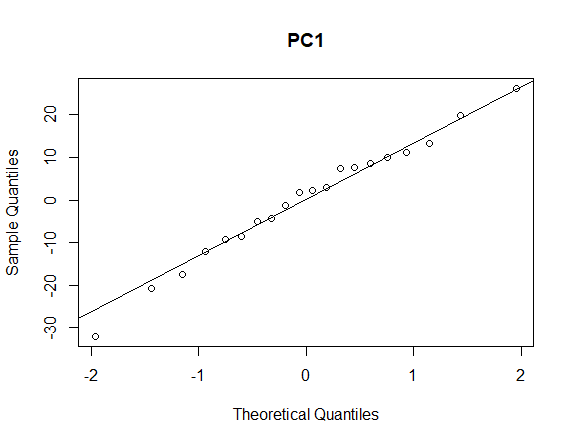
\includegraphics[scale=0.8]{QQplot.png}
		\caption{Q-Q plot}
	\end{figure}

\end{answer}
\end{document}